%   Filename    : chapter_4.tex 

\chapter{Results and Discussions}
This chapter presents the results of the machine learning and deep learning analyses conducted on the preprocessed dataset. Preprocessing was performed using Python in Google Colaboratory. The chapter includes the evaluation of various machine learning classifiers, analysis of feature importance, and the application of deep learning models for image-based classification. These approaches aim to identify key predictors and assess classification performance for sex identification in \textit{T. granosa}.

\section{Machine Learning Analysis}
\subsection{Data Exploration}

\begin{figure}[!htbp]
	\centering
	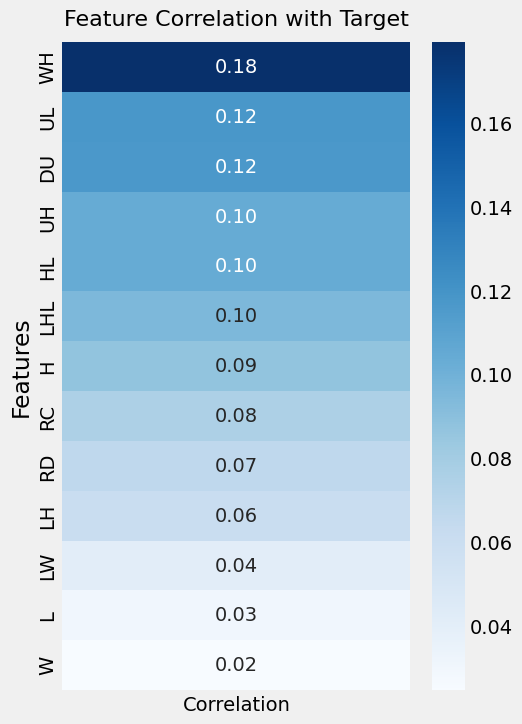
\includegraphics[width=0.4\textwidth]{figures/heatmap.png}
	\caption{Correlation heatmap of morphometric features with the sex of \textit{T. granosa}}
	\label{fig:heatmap}
\end{figure}

Exploratory data analysis was performed to characterize the dataset using visualizations to understand the patterns and correlations within the data. A correlation heatmap was created to assess the relationship between the predictors and the target variable.

The heatmap (see Figure~\ref{fig:heatmap}) revealed three features most correlated with the sex of \textit{T. granosa}: the width-height ratio (r = 0.18), the umbos-length ratio (r = 0.12), and the distance between the umbos (r = 0.12). Each of these features demonstrated a weak positive relationship with the target variable. 

\subsection{Statistical Analysis}

\begin{table}[H]
	\centering
	\small % or \footnotesize or \scriptsize
	\begin{tabular}{lc}
		\hline
		\textbf{Variable} & \textbf{p-value} \\ \hline
		Length & 0.334 \\
		Width & 0.753 \\
		Height & 0.124 \\
		Rib count & 0.251 \\
		Length (Hinge Line) & 0.120 \\
		Distance Umbos & 0.025 \\
		LW\_ratio & 0.011 \\
		LH\_ratio & 0.490 \\
		WH\_ratio & 0.003 \\
		UL\_ratio & 0.019 \\
		HL\_ratio & 0.079 \\
		UH\_ratio & 0.036 \\
		Rib Density & 0.181 \\ \hline
	\end{tabular}
	\caption{Mann-Whitney U Test Results for Sex-Based Feature Comparison}
	\label{tab:mann-whitney}
\end{table}

As part of the exploratory data analysis, statistical testing confirmed that the dataset did not follow a normal distribution. Consequently, the Mann-Whitney U test was applied with a significance level of $\alpha = 0.05$ to compare male and female samples. Out of thirteen features, five showed statistically significant differences. These included: distance between umbos ($p = 0.025$), length-width ratio ($p = 0.011$), umbos-length ratio ($p = 0.019$), width-height ratio ($p = 0.003$), and umbos-height ratio ($p = 0.036$). 

It is important to note that statistical significance does not imply predictive importance. Therefore, further analysis—such as feature importance evaluation—was performed to identify the most informative predictors for classification.

\subsection{Feature Importance Analysis}

\begin{figure}[!htbp]
	\centering
	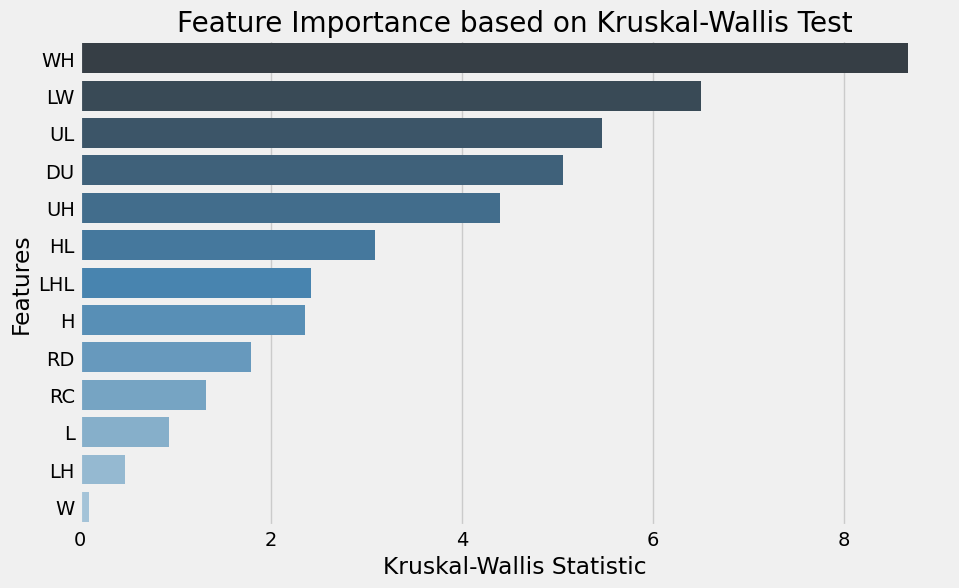
\includegraphics[width=1.0\textwidth]{figures/kw.png}
	\caption{Feature Importance Scores Using the Kruskal-Wallis Test}
	\label{fig:kw}
\end{figure}

Feature importance was assessed using the Kruskal-Wallis test, a non-parametric method that is suitable for evaluating differences in distributions across groups when the data does not follow a normal distribution. This approach was chosen because of the non-normality of the dataset and its robustness in handling continuous and ordinal data without assuming homogeneity of variances. \cite{ribeiro2024}

The analysis showed that the width-to-height ratio (WH\_ratio) had the highest importance score, indicating it is the most statistically significant feature for distinguishing the sex of \textit{T. granosa}. Other notable features included the length-to-width ratio (LW\_ratio), umbos-to-length ratio (UL\_ratio), and the distance between the umbos, all of which contributed significantly to the classification task.

\subsection{Performance Evaluation}

\begin{table}[H]
	\centering
	\resizebox{\textwidth}{!}{
		\begin{tabular}{lcccccc}
			\hline
			\textbf{Model} & \textbf{Accuracy (\%)} & \textbf{Precision (\%)} & \textbf{Recall (\%)} & \textbf{F1-Score (\%)} \\ \hline
			Support Vector Machine   & 64.89 & 65.88 & 64.89 & 64.22 \\
			Logistic Regression      & 64.50 & 65.37 & 64.50 & 63.85 \\
			K-Nearest Neighbors      & 64.14 & 64.52 & 64.14 & 63.99 \\
			Extra Trees              & 63.75 & 63.22 & 62.96 & 62.84 \\
			Random Forest            & 62.96 & 60.81 & 60.59 & 60.38 \\
			Gradient Boosting        & 62.56 & 63.26 & 62.56 & 62.22 \\
			AdaBoost                 & 60.60 & 61.39 & 60.60 & 60.03 \\
			\hline
		\end{tabular}
	}
	\caption{Performance Metrics for Models with 2 Features}
	\label{tab:performance-2-features}
\end{table}

Table~\ref{tab:performance-2-features} presents the performance metrics of various machine learning models when trained using only the two most informative features, as identified through feature selection. The evaluation metrics—accuracy, precision, recall, and F1-score—collectively provide a comprehensive view of each model's ability to correctly classify the sex of \textit{T. granosa} specimens.

Interestingly, despite the simplicity of using only two features, this configuration yielded the highest classification performance across all feature sets. Among the models, the Support Vector Machine (SVM) achieved the best results, with an accuracy of 64.89\%, precision of 65.88\%, recall of 64.89\%, and an F1-score of 64.22\%. Logistic Regression and K-Nearest Neighbors (KNN) also performed competitively, with F1-scores of 63.85\% and 63.99\%, respectively.

In contrast, ensemble-based models such as Random Forest, Gradient Boosting, and AdaBoost demonstrated slightly lower performance, potentially due to the limited number of features restricting their ability to capture complex patterns and interactions typically leveraged by such models.

It is important to note that these machine learning models were also trained using the full set of 13 features and an intermediate set of 5 features, as detailed in Table~4.1. Surprisingly, the two-feature configuration outperformed both larger feature sets across most models. This finding underscores the value of effective feature selection, suggesting that simpler models with fewer inputs can sometimes yield better generalization and performance than more complex configurations. Moreover, reducing the number of features has practical advantages in terms of data collection, model interpretability, and computational efficiency.